\documentclass[12pt,letterpaper]{article}
\usepackage{graphicx,textcomp}
\usepackage{natbib}
\usepackage{setspace}
\usepackage{fullpage}
\usepackage{color}
\usepackage[reqno]{amsmath}
\usepackage{amsthm}
\usepackage{fancyvrb}
\usepackage{amssymb,enumerate}
\usepackage[all]{xy}
\usepackage{endnotes}
\usepackage{lscape}
\newtheorem{com}{Comment}
\usepackage{float}
\usepackage{hyperref}
\newtheorem{lem} {Lemma}
\newtheorem{prop}{Proposition}
\newtheorem{thm}{Theorem}
\newtheorem{defn}{Definition}
\newtheorem{cor}{Corollary}
\newtheorem{obs}{Observation}
\usepackage[compact]{titlesec}
\usepackage{dcolumn}
\usepackage{tikz}
\usetikzlibrary{arrows}
\usepackage{multirow}
\usepackage{xcolor}
\newcolumntype{.}{D{.}{.}{-1}}
\newcolumntype{d}[1]{D{.}{.}{#1}}
\definecolor{light-gray}{gray}{0.65}
\usepackage{url}
\usepackage{listings}
\usepackage{color}

\definecolor{codegreen}{rgb}{0,0.6,0}
\definecolor{codegray}{rgb}{0.5,0.5,0.5}
\definecolor{codepurple}{rgb}{0.58,0,0.82}
\definecolor{backcolour}{rgb}{0.95,0.95,0.92}

\lstdefinestyle{mystyle}{
	backgroundcolor=\color{backcolour},   
	commentstyle=\color{codegreen},
	keywordstyle=\color{magenta},
	numberstyle=\tiny\color{codegray},
	stringstyle=\color{codepurple},
	basicstyle=\footnotesize,
	breakatwhitespace=false,         
	breaklines=true,                 
	captionpos=b,                    
	keepspaces=true,                 
	numbers=left,                    
	numbersep=5pt,                  
	showspaces=false,                
	showstringspaces=false,
	showtabs=false,                  
	tabsize=2
}
\lstset{style=mystyle}
\newcommand{\Sref}[1]{Section~\ref{#1}}
\newtheorem{hyp}{Hypothesis}

\title{Problem Set 2}
\date{Due: October 15, 2023}
\author{Applied Stats/Quant Methods 1}

\begin{document}
	\maketitle
	\section*{Instructions}
\begin{itemize}
	\item Please show your work! You may lose points by simply writing in the answer. If the problem requires you to execute commands in \texttt{R}, please include the code you used to get your answers. Please also include the \texttt{.R} file that contains your code. If you are not sure if work needs to be shown for a particular problem, please ask.
	\item Your homework should be submitted electronically on GitHub.
	\item This problem set is due before 23:59 on Sunday October 15, 2023. No late assignments will be accepted.

\end{itemize}

	
	\vspace{.5cm}
	\section*{Question 1: Political Science}
		\vspace{.25cm}
	The following table was created using the data from a study run in a major Latin American city.\footnote{Fried, Lagunes, and Venkataramani (2010). ``Corruption and Inequality at the Crossroad: A Multimethod Study of Bribery and Discrimination in Latin America. \textit{Latin American Research Review}. 45 (1): 76-97.} As part of the experimental treatment in the study, one employee of the research team was chosen to make illegal left turns across traffic to draw the attention of the police officers on shift. Two employee drivers were upper class, two were lower class drivers, and the identity of the driver was randomly assigned per encounter. The researchers were interested in whether officers were more or less likely to solicit a bribe from drivers depending on their class (officers use phrases like, ``We can solve this the easy way'' to draw a bribe). The table below shows the resulting data.

\newpage
\begin{table}[h!]
	\centering
	\begin{tabular}{l | c c c }
		& Not Stopped & Bribe requested & Stopped/given warning \\
		\\[-1.8ex] 
		\hline \\[-1.8ex]
		Upper class & 14 & 6 & 7 \\
		Lower class & 7 & 7 & 1 \\
		\hline
	\end{tabular}
\end{table}

\begin{enumerate}
	
	\item [(a)]
	Calculate the $\chi^2$ test statistic by hand/manually (even better if you can do "by hand" in \texttt{R}).\\
	\vspace{1cm}
	\lstinputlisting[language=R, firstline=3, lastline=44]{P02_my_answers_daijin_zhou.R}
	\noindent
	- Results: the square of X is 3.17.
	\item [(b)]
	Now calculate the p-value from the test statistic you just created (in \texttt{R}).\footnote{Remember frequency should be $>$ 5 for all cells, but let's calculate the p-value here anyway.}  What do you conclude if $\alpha = 0.1$?\\
	\vspace{1cm}
	\lstinputlisting[language=R, firstline=46, lastline=54]{P02_my_answers_daijin_zhou.R}
	\noindent
	- Results: because p value is 0.15 which is  higher than 0.1, we need to accept H0. There is no significant association between the variables.
	\item [(c)] Calculate the standardized residuals for each cell and put them in the table below.
	\begin{table}[h]
		\centering
		\begin{tabular}{l | c c c }
			& Not Stopped & Bribe requested & Stopped/given warning \\
			\\[-1.8ex] 
			\hline \\[-1.8ex]
			Upper class  & 0.322 & -1.644 & 1.523 \\
			\\
			Lower class & -0.322 & 1.642  & -1.523  \\
			
		\end{tabular}
	\end{table}
	\vspace{1cm}
    \lstinputlisting[language=R, firstline=56, lastline=69]{P02_my_answers_daijin_zhou.R}  		
	
	\vspace{1cm}
	\item [(d)] How might the standardized residuals help you interpret the results?\\  
	\noindent
	- Results:\\
	The standardized residual between "Upper class"and "Not Stopped" is 0.322.  Because it is close to zero, it suggests that the observed and expected frequencies are close, and there may not be a strong association between  "Upper class" and "Not Stopped".\\
	
	
	The standardized residual between "Upper class"and "Bribe requested" is -1.644.  Because it is negative, it suggests the observed frequency of "Upper class" individuals requesting a bribe is lower than what would be expected. It suggests that "Upper class"  might not likely to request a bribe.\\
	
	
	The standardized residual between "Upper class"and "Stopped/given warningd" is 1.523.  Because it is a positive value.This suggests that the observed frequency of "upper-class" individuals being stopped is higher than expected. It suggests that "Upper class"  might be likely to be stopped.\\
	
	
	The standardized residual between "Lower class"and "Not Stopped" is -0.322.  Because it is close to zero, it suggests that the observed and expected frequencies are close, and there may not be a strong association between  "Lower class" and "Not Stopped".\\
	
	
	The standardized residual between "Lower class"and "Bribe requested" is 1.642.  Because it is a positive value.This suggests that the observed frequency of "Lower class" individuals being stopped is higher than expected. It suggests that "Lower class"  might be likely to request a bribe. \\
	
	
	The standardized residual between "Lower class"and "Stopped/given warning" is -1.532.  Because it is negative, it suggests the observed frequency of "Lower class" individuals being stopped is lower than expected.  It suggests that "Lower class"  might not likely to be stopped.\\
\end{enumerate}

\section*{Question 2: Economics}
Chattopadhyay and Duflo were interested in whether women promote different policies than men.\footnote{Chattopadhyay and Duflo. (2004). ``Women as Policy Makers: Evidence from a Randomized Policy Experiment in India. \textit{Econometrica}. 72 (5), 1409-1443.} Answering this question with observational data is pretty difficult due to potential confounding problems (e.g. the districts that choose female politicians are likely to systematically differ in other aspects too). Hence, they exploit a randomized policy experiment in India, where since the mid-1990s, $\frac{1}{3}$ of village council heads have been randomly reserved for women. A subset of the data from West Bengal can be found at the following link: \url{https://raw.githubusercontent.com/kosukeimai/qss/master/PREDICTION/women.csv}\\

\noindent Each observation in the data set represents a village and there are two villages associated with one GP (i.e. a level of government is called "GP"). Figure~\ref{fig:women_desc} below shows the names and descriptions of the variables in the dataset. The authors hypothesize that female politicians are more likely to support policies female voters want. Researchers found that more women complain about the quality of drinking water than men. You need to estimate the effect of the reservation policy on the number of new or repaired drinking water facilities in the villages.
\vspace{.5cm}
\begin{figure}[h!]
	\caption{\footnotesize{Names and description of variables from Chattopadhyay and Duflo (2004).}}
	\vspace{.5cm}
	\centering
	\label{fig:women_desc}
\end{figure}		

\newpage
\begin{enumerate}
	\item [(a)] State a null and alternative (two-tailed) hypothesis.\\ 
	\noindent 
	Null Hypothesis (H0):
	The reservation policy for women leaders in village has no effect on the number of new or repaired drinking water facilities in the villages.
	\vspace{1cm}
	\noindent\\ 
	Alternative Hypothesis (H1):
	The reservation policy for women leaders has a significant effect on the number of new or repaired drinking water facilities in the villages.
	\vspace{1cm}
	\item [(b)] Run a bivariate regression to test this hypothesis in \texttt{R} (include your code!).
	\lstinputlisting[language=R, firstline=82, lastline=95]{P02_my_answers_daijin_zhou.R}
	\vspace{1cm}
	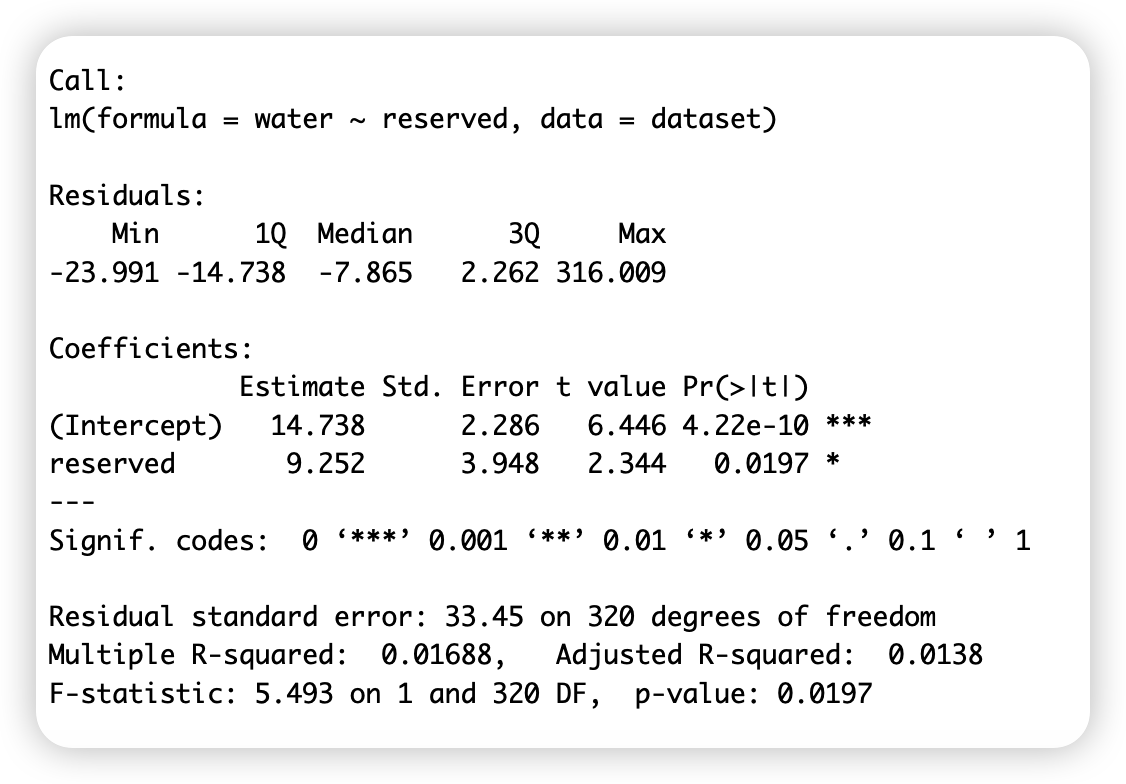
\includegraphics[width=0.99\textwidth]{P02_my_answers_daijin_zhou.png}
	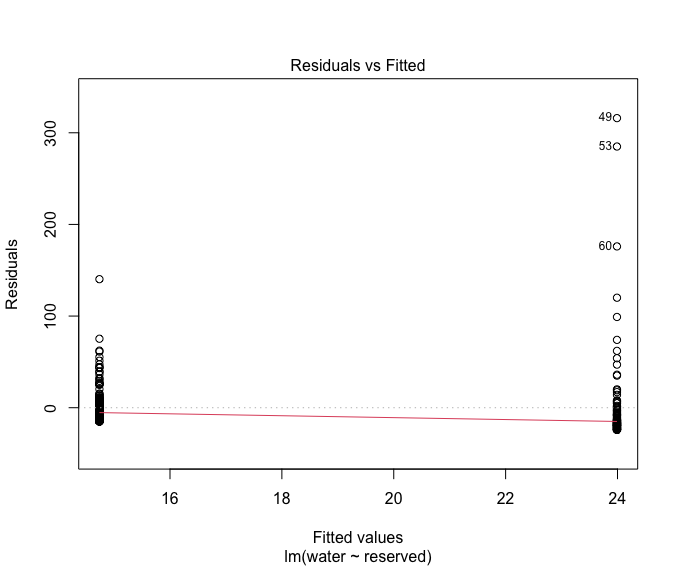
\includegraphics[width=0.99\textwidth]{P02_my_answers_daijin_zhou_2b.png}
	\item [(c)] Interpret the coefficient estimate for reservation policy. 
	\noindent\\
    - Results:\\
    Coefficient Value: 
    The positive coefficient estimate of 9.252 suggests that when the village council head's position is reserved for women, there is an increase by 9.252 on the number of new or repaired drinking water facilities compaired to situations with no reservation policy.\\
    
    Statistical Significance: The p-value of 0.0197 suggests statistical significance which is smaller than threshold of 0.05. This suggests that the implementation of a reservation policy has a significant impact on the number of new or repaired drinking water facilities.
\end{enumerate}

\end{document}
